
\documentclass{report}
\usepackage{hyperref}
\usepackage{graphicx}
\usepackage{gensymb}
\usepackage{multirow}
\usepackage{longtable}
\usepackage{color}

% Setting up hyperrefs	
\hypersetup{        % show bookmarks bar?
    unicode=false,          % non-Latin characters in Acrobat’s bookmarks
    pdftoolbar=true,        % show Acrobat’s toolbar?
    pdfmenubar=true,        % show Acrobat’s menu?
    pdffitwindow=false,     % window fit to page when opened
    pdfstartview={FitH},    % fits the width of the page to the window
    pdftitle={Atlantis User Guide},    % title
    pdfauthor={Author},     % author
    pdfsubject={Subject},   % subject of the document
    pdfcreator={Creator},   % creator of the document
    pdfproducer={Producer}, % producer of the document
    pdfkeywords={keyword1} {key2} {key3}, % list of keywords
    pdfnewwindow=true,      % links in new window
    colorlinks=false,       % false: boxed links; true: colored links
    linkcolor=red,          % color of internal links (change box color with linkbordercolor)
    citecolor=green,        % color of links to bibliography
    filecolor=magenta,      % color of file links
    urlcolor=cyan           % color of external links
}
\usepackage[style=numeric,backend=biber]{biblatex}
\addbibresource{hi_literature.bib}

\begin{document}
\title{Atlantis (Iceland) User Guide}
\author{Christopher David Desjardins}
\date{\today}
\maketitle
\newpage

\tableofcontents
\newpage

\chapter{Preface}

\begin{table}[!htbp]
\caption{Atlantis Terminology}
\begin{tabular}{lp{10cm}}
\hline
BGM & Box Geometry Model. This is the file format that Atlantis requires its spatial file in. This can be converted using their \texttt{bgmeriser} java tool to convert a *.shp to a *.bgm. The requires projection information in order to account for latitudinal differences in daylength and for visualization. \\
\hline
\end{tabular}
\end{table}


\chapter{Introduction to Atlantis}

\newpage
\section{Setting up the spatial data}

Atlantis requires a special spatial file format. This is termed a bgm file (box geometry file). The bgm defines the geography (i.e.\ bathmetry) used in the Atlantis model. The bgm file stores the saptial information in x and y terms rather than latitude and longitude. Information about the projection (which is used in visualization and for determining daylength), number of boxes, number of dynamic faces, maximum depth, vertical mixing and horizontal transport scalars, whether a box is a boundary box (i.e.\ is it dynamic, meaning does it border the open ocean) and spatial layout of the boxes and faces (e.g.\ area, location of vertices, depth of box) is specified in the bgm file. 

 For the Icelandic Atlantis model, data contained in the
 \texttt{reitmapping.tsv} and the \texttt{R} \texttt{geo} package were
 used to develop the spatial layer. The subdivisions used are
 described in \cite{dst2}. The subdivisions were exported from
 \texttt{R} to \texttt{QGIS} where they were modified to not overlap
 with Iceland, Greenland, and the Faroe Islands and boundary boxes
 were added around the subdivisions. The boundary boxes, generally,
 buffer the active model area by $1/2\degree$ longitude and
 $1/4\degree$ latitude. The spatial map is shown in figure~\ref{ref:spdef}. Comparing figure with the figure 9.7 in
 \cite{dst2}, the location and, generally, uniform width of the
 boundary box around the subdivisions is discernible. 

On the CSIRO wiki, there are various tools to help create a bgm file. In particular the \texttt{bgmeriser.jar} tool was used after the shapefile was cleaned in \texttt{QGIS} and \texttt{GRASS}. The projection used was ISN93/Lambert 1993, which corresponds to the following \texttt{proj4} format:   

\begin{small}
\begin{verbatim}
+proj=lcc +lat_1=64.25 +lat_2=65.75 +lat_0=65 +lon_0=-19 +x_0=500000 
+y_0=500000 +ellps=GRS80 +towgs84=0,0,0,0,0,0,0 +units=m +no_defs 
\end{verbatim}
\end{small}

This was the projection information was obtained from \cite{proj4iceland} and provided to the \texttt{bgmeriser.jar} tool.

 The maximum depth for the boxes shown in figure~\ref{ref:spdef} was based on the depth information provided in \texttt{geo::gbdypi}. The depths ranged from 100m to 3800m, exluding Iceland the Faroe Islands which are assigned a depth of 0 in the model (to avoid having islands in the bgm file).
 
 For the Icelandic Atlantis model, the water column was split up into at most six layers: 0 - 50 m, 50 - 150 m, 150 - 300 m, 300 - 600m, 600 - 1000m, 1000m). The size of these layers was selected after consultation with researchers at Hafro and these layers are similar to depth layers used in other Atlantis models \cite{link2010northeast, savina2008ecologically}.


\begin{center}
\begin{figure}
\caption{Spatial Defintions of the Atlantis Iceland model}
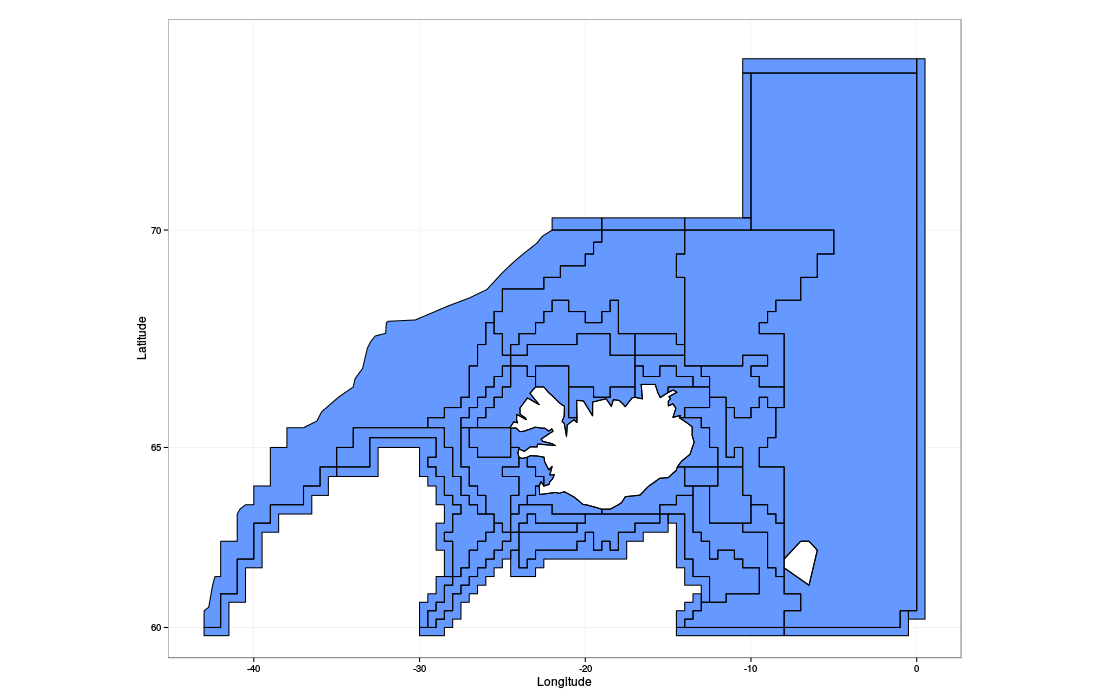
\includegraphics[scale=.3]{maps/atlantis_iceland_WGS84.png}
\label{ref:spdef}
\end{figure}
\end{center}

\section{Initial Conditions cdf}

The initial conditions cdf (init.cdf) contains the values to initialize the functional group tracers as well as some other tracers (e.g. nitrification, oxygen) that are required for the model. Table ~\ref{tab:init} shows the flags used in the init.cdf file.

\begin{center}
\begin{longtable}{llp{8cm}}
\caption{Flags set in the \texttt{init.cdf} file} \\
\hline
Flag & Values & Description \\
\hline
\multirow{3}{*}{bmtype} & ``tracer"  & tracer are variables we track and are dynamic and not epibenthic \\ 
&  ``phys" &  physical variables are static \\
& ``epibenthos" & variables that occur in the epibenthos \\
\hline
\multirow{20}{*}{unit} & ``mg N m-3" & Nitrogen unit for organisms occurring in the water column i.e.\ (t, b, z) \\
&``mg N m-2" & Nitrogen unit for organisms occurring in the epibenthos i.e.\ (t, b) \\
&``mg N" & Nitrogen unit for residual weight and structural weight for vertebrates \\
&``1" & Abundance, i.e.\ number of individuals, relevant only for vertebrates OR for some of the hydrographic tracers (e.g.\ percent canyon) \\
&``m" & Meters, relevant for some physical variables (e.g.\ max depth of detritus) \\
&`` " & Unitless, e.g.\ number of layers \\
&``m s-1" & Meters per second, relevant for erosion\_rate \\
&``m3" & Cubic meters, for volume of the layer \\
&``PSU" & Practical salinity units, relevant for salinity \\
&``Animals per m2" & Unit for the biological activity phys \\
&``**U" & Light adaption for tracers with \texttt{isCover = 1} in the \texttt{functionalGroup.csv}, replace ** with \texttt{Code} in \texttt{functionalGroup.csv}  \\
&``mg Si m$-$3" & mg of Silicon per cubic meter for tracers that have \texttt{isSiliconDep = 1} in the \texttt{functionalGroup.csv} \\
\hline
long\_name & Any Character & This is the long name of the variable from the \texttt{functionalGroup.csv} \\
\hline
sumtype & 0 or 1  & Flag to indicate whether summary data type  \\
\hline
dtype & 0 or 1 & Flag for general data type, if fisheries data than 1. \\
\hline
inwc & 0 or 1 & Flag whether exists in water column, depends on \texttt{GroupType} in \texttt{functionalGroup.csv} \\
\hline
insed & 0 or 1 & Flag whether exists in sediment, depends on \texttt{GroupType} in \texttt{functionalGroup.csv} \\
\hline
dissol & 0 or 1 & Flag whether dissolved or not \\
\hline
decay & Any Non-Negative Numeric & Decay constant \\
\hline 
partic & 0 or 1 & Flag whether particulate or not. On for all in \texttt{functionalGroup.csv} by default \\
\hline 
passive & 0 or 1 & Flag indicating whether group is active or passive with regard to advection and movement with currents \\
\hline
svel & Any Non-Negative Numeric & Settling constant \\ 
\hline
xvel & Any Non-Negative Numeric & Extra "settling" velocity due to migration or nutrient limitation. Default to 0. \\
\hline
psize & Any Non-Negative Numeric & Particle size \\
\hline
b\_dens & 1000000000. & Particle bulk density. Atlantis defualts to 1000000000. \\
\hline
i\_conc & 200000000. & Initial deposit concentration. Atlantis defaults to 200000000. \\
\hline
f\_conc & 200000000. & Compacted deposit concentration. Atlantis defaults to 200000000. \\
\hline
\_FillValue & Any Non-Negative Number & What value should the model fill in if missing, i.e.\ if  ``\_" \\
\hline
:title & &  Description of this data set \\
\hline
:geometry  & & Name of geometry file \\
\hline
:parameters  & & Name of parameter file \\
\hline
:wcnz & & Number of water column layers \\
\hline
:sednz & & Number of sediment layers \\
\hline
\label{tab:init}
\end{longtable}
\end{center}





\section{Fleet Structure}

\section{Setting up Atlantis for Iceland}

\subsection{Functional Group Definition File}

Initially, the groups set up in the functional group definition file came from the MRI's State of Marine Stocks in Icelandic Waters 2012/2013, Prospects for the Quota Year 2013/2014 report. Namely from Tables 1 and 2, where MRI provides advice for the quotas 2013/2014. In addition, other marine fauna and flora listed on the Ministry of Fisheries website \cite{is_fish} and FishBase \cite{fishdb} where included as a functional groups. 

\subsection{Data Requirements}

Data requirements are taken, initially, from Kaplan (2007) notes on the Atlantis wiki.

\subsubsection{Primary Producers}

Primary producer abundance is modeled as an aggregrated biomass pool in each spatial box. The model tracks (mg N/m$^3$) per box. Growth is governed by the following equation:

\begin{equation}
\frac{d(PX_w)}{dt} = G_{PX_w} - M_{lys,PX} - M_{lin} - M_{quad} - \sum_{i = pred groups}{P_{PX_{w,i}}}
\end{equation}

Where $G_{PX_w}$ is defined as

\begin{equation}
G_{PX} = \mu_{PX} * \delta_{irr} * \delta_{N} * \delta{space} * PX
\end{equation}

$G_{PX}$ then stands for the growth of PX, $M_{lys,PX}$ is the loss of PX due to lysis, $M_{lin}$ and $M_{quad}$ are loss due to linear and quadratic mortality, $P_{PX,I}$ are the losses of PX due to depredation, $\mu_{PX}$ is the maximum growth rate, and $\delta_{irr}, \delta_{N},$ and $\delta{space}$ are light, nutrient and space limitation. 

\subsubsection{Invertebrates}

Invertebrates are also modeled as aggregated biomass pools in each spatial cell and abundance (mg N/m$^3$) per box is tracked based on growth, depredation, and linear and quadratic mortality. The linear and quadratic mortality represent ecological components not treated explicitly in the model and linear and quadratic mortality are density independent and density dependent effects, respectively. 

\subsubsection{Vertebrates}

Vertebrates are represented as 10 age classes. These age classes represent distinct life cycles that the organism passes through. The duration of each age class is always 10\% of the total longevity of the organism. 

For each age class and each spatial cell, the model tracks the number of individuals, their average structural weight (bones and hard parts, in mg N/m$^3$), and reserve weight (soft tissue, mg N/mg$^3$). Growth and abundance are governed by functions of recruitment, depredation, consumption, and linear and quadratic mortality. Atlantis tracks abundance, biomass, weight-at-age, and condition (reserve weight/structural weight) of each group through time, in each box, and for the entire model domain.

\subsection{Nutrients}  


\section{Additional Iceland Information}

\subsection{Cod}
In 2010 reference points of $B_{trigger}$ and $B_{lim}$ were determined for cod. These are relative to the spawning stock and $B_{trigger} = 220$ thousand tonnes and $B_{lim} = 125$ thousand tonnes (based on the historical minimum). 

\subsection{Haddock}
In 2013 reference points of $B_{trigger}$ and $B_{lim}$ were determined for haddock related to the spawning stock. These were both set to 45 thousand tonnes (i.e.\ the historical minimum).

\subsection{Saithe}

The management plan is based on a harvest control rule (HCR) that sets the TAC for the coming quota year as the average of the previous year’s TAC and 20\% of the current reference biomass. If the spawning stock drops below the reference point $B_{trigger}$ (65 thous. tonnes) the harvest rate is decreased. This HCR will lead to smaller fluctuations in TAC from year to year, compared to fluctuations in the stock assessment.

\subsection{Phytoplankton}


\section{Astthorsson et al. (2007). Climate variability and the Icelandic marine ecosystem}
Diatoms of the genera \textit{Thalassiosira} spp. and \textit{Chaetoceros} spp. typically dominate the phytoplankton spring bloom. Dinoflagellates of the genera \textit{Ceratium} spp. and \textit{Protoperidinium} spp. increase in abundance after the spring bloom while diatoms continue to be relatively abundant

\subsection{Google Drive}

              
Atlantis Notes

Model Components
At the core of Atlantis is a deterministic biophysical sub-model, coarsely spatially-resolved in three dimensions, which tracks nutrient (usually N and S$_i$) flows through the main biological groups in the system. The primary ecological processes modelled are consumption, production, waste production, migration, predation, recruitment, habitat dependency, and mortality. The trophic resolution is typically at the functional group level. Invertebrates are typically represented as biomass pools, while vertebrates are represented using an explicit age-structured formulation. The physical environment is also represented explicitly, via a set of polygons matched to the major geographical and bioregional features of the simulated marine system. Biological model components are replicated in each depth layer of each of these polygons. Movement between the polygons is by advective transfer or by directed movements depending on the variable in question.

Atlantis also includes a detailed industry (or exploitation) sub-model. This model deals not only with the impact of pollution, coastal development and broad-scale environmental (e.g. climate) change, but is focused on the dynamics of fishing fleets. It allows for multiple fleets, each with its own characteristics of gear selectivity, habitat association, targeting, effort allocation and management structures. At its most complex, it includes explicit handling of economics, compliance decisions, exploratory fishing and other complicated real world concerns such as quota trading. All forms of fishing may be represented, including recreational fishing (which is based on the dynamically changing human population in the area).

The exploitation model interacts with the biotic part of the ecosystem, but also supplies ‘simulated data’ to the sampling and assessment sub-model. The sampling and assessment sub-model in Atlantis is designed to generate sector dependent and independent data with realistic levels of measurement uncertainty evaluated as bias and variance. These simulated data are based on the outputs from the biophysical and exploitation sub-models, using with a user-specified monitoring scheme. The data are then fed into the same assessment models used in the real world, and the output of these is input to a management sub-model. This last sub-model is typically a set of decision rules and management actions (currently only detailed for the fisheries sector), which can be drawn from an extensive list of fishery management instruments, including: gear restrictions, days at sea, quotas, spatial and temporal zoning, discarding restrictions, size limits, bycatch mitigation, and biomass reference points.


Useful References
Kaplan, I.C., Levin P.S., Burden M. and Fulton, E.A., in press. Fishing Catch Shares in the Face of Global Change: A Framework for Integrating Cumulative Impacts and Single Species Management. Canadian Journal Fisheries and Aquatic Sciences.

Link, J.S., Fulton, E.A. and Gamble, R.J. in press. The Northeast US Application of ATLANTIS: An full system model exploring marine ecosystem dynamics in a living marine resource management context. Progress in Oceanography

Fulton, E.A., Smith A.D.M., Smith D.C. and van Putten, I.E., 2010. Human behaviour - the neglected source of uncertainty in fisheries management. Fish and Fisheries. DOI: 10.1111/j.1467-2979.2010.00371.x

Fulton, E.A., 2010. Approaches to end to end ecosystem models. Journal of Marine Systems. doi:10.1016/j.jmarsys.2009.12.012 


Fulton, E.A., Smith, A.D.M. and Smith, D.C., 2007. Alternative Management Strategies for Southeast Australian Commonwealth Fisheries: Stage 2: Quantitative Management Strategy Evaluation. Australian Fisheries Management Authority Report. (9 MB pdf)

Fulton E. A., Smith, A. D. M., and Punt, A. E., 2005. Which ecological indicators can robustly detect effects of fishing? ICES Journal of Marine Science 62:540 – 551.

The Atlantis framework, developed from the ‘‘Bay Model 2’’ ecosystem model (Fulton et al., 2004a), is a deterministic model that tracks the nutrient (nitrogen and silica) flow through the main biological groups found in temperate marine ecosystems (Table 1), and three detritus
groups (labile detritus, refractory detritus, and carrion). The invertebrate and primary producer groups are simulated using aggregate biomass pools, while the vertebrates are
represented through age-structured models.

The main biological groups that need to be included are:

(i) groups with fast turnover rates (e.g. phytoplankton, zooplankton, bacteria) that, while non-selective (they do not only respond to fisheries-induced perturbations), will nevertheless respond quickly to any change in the system (such groups may cause false alerts, but react sufficiently fast to be potentially useful as early warning indicators);

(ii) groups that are targeted by fisheries (they can usefully summarize the current status of that part of the foodweb of most interest to humans);

(iii) habitat-defining groups (particularly in coastal ecosystems, because they have critical roles in
benthic communities and are often a good proxy for overall biodiversity levels);

(iv) charismatic (or sensitive) groups (often found at the top of the foodweb, such groups usually have slow dynamics and can convey information about the underlying system state, and how heavily it has been impacted by fishing).



\cite{fulton2003effect}
This paper is a review of the extent ecological models. Ultimately it concludes by stating there is much work to be done in this area and that there is an important trade off between simplicity and complexity. 


Iceland Ecosystem Modeling

\cite{bormicon}

The interaction of cod and capelin form the impetus of the Bormicon report.

Capelin most important prey of Icelandic cod. 

Variability in the Atlantic inflow causes considerable interannual differences in temperature and salinity

Cod and capelin spawn off the S or SW coast in March - May and eggs and larvae drift along west coast to nursery areas off the N and E coast. 

Figure 2.2.1 and 2.2.2? Which is salinity and which is temperature? Is there a Non-Negative relationship btwn the two?

Cod
Spawn off S coast, eggs drift CW to nurseries off N coast

Mortality - fishing, cannibalism, and natural mortality (i.e. marine mammals, diseases, other fish, and invertebrates - depending upon life cycle)

Annual survey, especially ground fish survey in March (is this still current??)

Capelin
 Spawn off S and W coast, eggs drift to N part around Iceland.

Immature capelin stay largely on the shelf, maturing portion return towards the northern part of the shelf in fall and migrates along the continental shelf edge, in a CW fashion to spawning groups in late March.

The larger part of each year-class matures and spawns at age 3, the remainder at age 4; there are few spawners aged 2 and 5-year-old spawners are very rare

Fishing mainly for reduction purposes.

Biological model
Separate fish into 0-group, immature, and mature fish.

Model unit of fish as the number of individuals of a given species within an area in a certain month, of the same age, length group, and maturity stage. 

Model migration, consumption, growth, and mortality.

Figure 3.1.1 provides the spatial definition of Icelandic waters based on bathymetry, hydrography, and biology. Are these spatial areas current? Has new information superseded this? This information differs from the spatial rectangles provided by Bjarki.

Bathymetry - depths
Hydrography - currents (i.e. upwellings, eddies, etc); temperature; salinity 

May not need to split up spatial rectangles based on distribution of fish species as we could say whether a particular species would use a particular vertical strata within a rectangle (differs from Bormicon?).

Cod are mainly caught at 0 - 500 m range.

Split to on-shelf and off-shelf parts

Shrimp may be an important prey to cod and the main fishery is located at depth ranging from 300 - 500 m. 

Greenland halibut off-shelf and fishery extends down to depths of 1500 m. 

Chapter 4 covers the mathematical functions used in Gadget to describe the events.

16 - 29 Jan 1994 survey. Cod stomachs containing capelin had a higher weight than those cod that didn’t consume capelin, cod feeding on the shelf area had higher stomach weights than cod feeding in the fjords. 

Cod and capelin distribution were overlapping to some extent, outside the fjord. 

Predator size of cod related to prey size of capelin, i.e. to some extent larger cod are consuming more large capelin than smaller capelin. 




Building the Atlantis Model

Step 1: BGM file - Spatial Data
Perhaps I need more data than what Bjarki sent? I at least need data on depth of the polygons.

Spatial Data
I believe that the data should have the following PROJ4 projection:
http://spatialreference.org/ref/epsg/3057/

atlantis friendly
%projection proj=lcc lat_1=64.25 lat_2=65.75 lat_0=65 lon_0=-19 x_0=500000 y_0=500000 ellps=GRS80 towgs84=0,0,0,0,0,0,0 units=m no_defs

%+proj=lcc +lat_1=64.25 +lat_2=65.75 +lat_0=65 +lon_0=-19 +x_0=500000 +y_0=500000 +ellps=GRS80 +towgs84=0,0,0,0,0,0,0 +units=m +no_defs

There can be no islands! Islands must be created as boxes with botz = 0. This can be accomplished with the Add Feature and enable snapping for only the layer of interest! Also might be useful to remove unnecessary vertices with the node tool but try to clean it first based on this instructions: https://wiki.csiro.au/display/Atlantis/Using+QGIS+to+clean+Atlantis+BGM+Shapefiles

Step 2: Force files
This seems to be very messy and will involve an exorbitant amount of time to create.







Icelandic Fisheries

ST5.3.3: Northern \& Western Waters – Iceland Waters. Lead: MRI. Participants: MRI, UI.
In the Icelandic case study a complex model incorporating the major stocks and fleets will be constructed. In the model the interactions between these stocks in terms of food interactions and mixed fisheries issues will be investigated. Stocks of lesser commercial importance such as tusk, ling, wolfish, plaice and marine mammals will be incorporated in the model. The impacts of changing stock dynamics on the whole system in terms of EAF will be a key importance in the case study.

3. Northern \& Western Waters – Icelandic Waters: species and data rich
In the Icelandic case study a complex GADGET model incorporating the major stocks and fleets will be constructed. In the model the interactions between these stocks in terms of food interactions and mixed fisheries issues will be investigated. The key species modelled are the gadoids; cod, haddock, saithe and the pelagic fish stocks such as capelin, herring and mackerel. Stocks of lesser commercial importance such as tusk, ling, wolffish and plaice will be incorporated as their productivity may be important in the highly mixed fishery in Icelandic
waters. Top predators such as whales and seals will be included in the model. The impacts of changing stock dynamics on the whole system in terms of EAFM will be of key importance in the case study. One Atlantis operating model will be based on the data from Icelandic waters.


Most krill species display large daily vertical migrations, thus providing food for predators near the surface at night and in deeper waters during the day.

\printbibliography[heading=bibintoc]

\chapter{Appendix}

\section{Literature Review}

\section{Miscellaneous}

To create the bgm the following command was run:

\begin{verbatim}
java -jar bgmeriser.jar -as "+proj=lcc +lat_1=64.25 +lat_2=65.75 +lat_0=65 +lon_0=-19 
+x_0=500000 +y_0=500000 +ellps=GRS80 +towgs84=0,0,0,0,0,0,0 +units=m +no_defs"
/path/to/shapefile_to_convert.shp
\end{verbatim}


\end{document}
